\documentclass[11pt,letterpaper]{article}

\usepackage[margin=0.6in]{geometry}
\usepackage{enumitem}
\usepackage{amsmath}
\usepackage{pgfplots}
\usetikzlibrary{decorations.pathmorphing, decorations.pathreplacing, calc}
\pgfplotsset{compat=1.15}
\usepackage{xcolor}
\newenvironment{solution}{\par\smallskip\color{blue!60!black}\textbf{Solution.}\ }{\par}

\pagestyle{empty}
\setlength{\parindent}{0pt}

\begin{document}

\begin{center}
    {\Large \textbf{16.07 Dynamics --- Quiz 1 Solutions: Spring-Loaded Inverted Pendulum}}
\end{center}


\begin{minipage}[t]{0.66\textwidth}


\vspace{14pt}
\begin{enumerate}[label=\textbf{\arabic*.}, leftmargin=*, itemsep=4pt, series=quiz]
\item The nonlinear equation of motion for the system shown is
\[
\ddot\theta = \frac{g}{\ell}\sin\theta - \frac{k}{m\ell^2}\,\theta .
\]
Find the critical stiffness $k_{cr}$, in terms of $m$, $g$, and $\ell$, at which the upright equilibrium transitions from stable to unstable.
\end{enumerate}
\end{minipage}%
\hfill
\begin{minipage}[t]{0.3\textwidth}
\vspace{0pt}
\centering
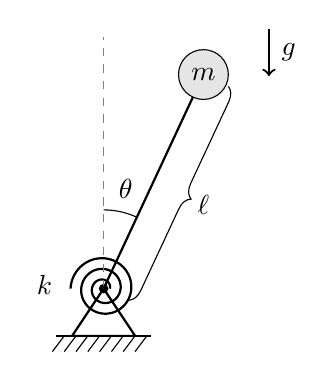
\begin{tikzpicture}[scale=1.0]
    \def\Lrod{3}
    \def\thetadeg{25}

    % --- Ground (fixed anchor) ---
    \draw[thick] (-0.6,-0.6) -- (0.6,-0.6);
    \foreach \x in {-0.5,-0.35,-0.2,-0.05,0.1,0.25,0.4,0.55}
        \draw (\x,-0.6) -- (\x-0.15,-0.8);

    % --- Support triangle (pin fixed to ground), apex at the pivot ---
    \draw[thick] (0,0) -- (-0.4,-0.6) -- (0.4,-0.6) -- cycle;

    % --- Torsion spring: flat spiral centered on the pivot ---
    \draw[thick] plot[domain=0:900, samples=150, variable=\t]
        ({(0.08+0.34*\t/900)*cos(\t)}, {(0.08+0.34*\t/900)*sin(\t)});
    \node at (-0.75,0.05) {$k$};

    % --- Pivot point ---
    \filldraw (0,0) circle (1.5pt);

    % --- Vertical reference (upright direction), dashed ---
    \draw[dashed, gray] (0,0) -- (0,3.2);

    % --- Rod at angle theta from vertical ---
    \coordinate (O) at (0,0);
    \coordinate (P) at ({\Lrod*sin(\thetadeg)},{\Lrod*cos(\thetadeg)});
    \draw[thick] (O) -- (P);

    % --- Mass at tip ---
    \filldraw[fill=gray!20] (P) circle (9pt);
    \node at (P) {$m$};

    % --- Angle arc, label centered on the arc ---
    \draw (0,1) arc (90:{90-\thetadeg}:1);
    \node at ({(1.3)*cos(90-\thetadeg/2)},{(1.3)*sin(90-\thetadeg/2)}) {$\theta$};

    % --- Length measurement: curly brace parallel to the rod, offset to its right ---
    \coordinate (Ob) at ({0.35*cos(\thetadeg)},{-0.35*sin(\thetadeg)});
    \coordinate (Pb) at ({\Lrod*sin(\thetadeg)+0.35*cos(\thetadeg)},{\Lrod*cos(\thetadeg)-0.35*sin(\thetadeg)});
    \draw[decorate, decoration={brace, amplitude=5pt, mirror}] (Ob) -- (Pb);
    \node at ($(Ob)!0.5!(Pb) + ({0.35*cos(\thetadeg)},{-0.35*sin(\thetadeg)})$) {$\ell$};

    % --- Gravity direction indicator ---
    \draw[->, thick] (2.1,3.3) -- (2.1,2.7);
    \node at (2.35,3.0) {$g$};
\end{tikzpicture}
\end{minipage}

\vspace{4pt}
\begin{enumerate}[label=\textbf{\arabic*.}, leftmargin=*, itemsep=10pt]
\item[] \begin{solution}
For small $\theta$, $\sin\theta \approx \theta$, so the linearized equation is
\[
\ddot\theta + \left(\frac{k}{m\ell^2} - \frac{g}{\ell}\right)\theta = 0 .
\]
If the coefficient is positive, solutions oscillate at $\omega_n = \sqrt{k/m\ell^2 - g/\ell}$ and the upright equilibrium is stable. If it is negative, solutions grow exponentially and the equilibrium is unstable. The transition happens when the coefficient is zero:
\[
\frac{k_{cr}}{m\ell^2} = \frac{g}{\ell} \quad\Longrightarrow\quad \boxed{k_{cr} = mg\ell}
\]
\end{solution}
\end{enumerate}

\begin{enumerate}[resume*=quiz, itemsep=10pt]

\item The plot below shows $U(\theta)$ for $k = 0.5\,k_{cr}$, with $m = \ell = 1$ and $g = 9.8$. Mark every stable equilibrium with a circle ($\circ$) and every unstable equilibrium with an $\times$.

\begin{center}
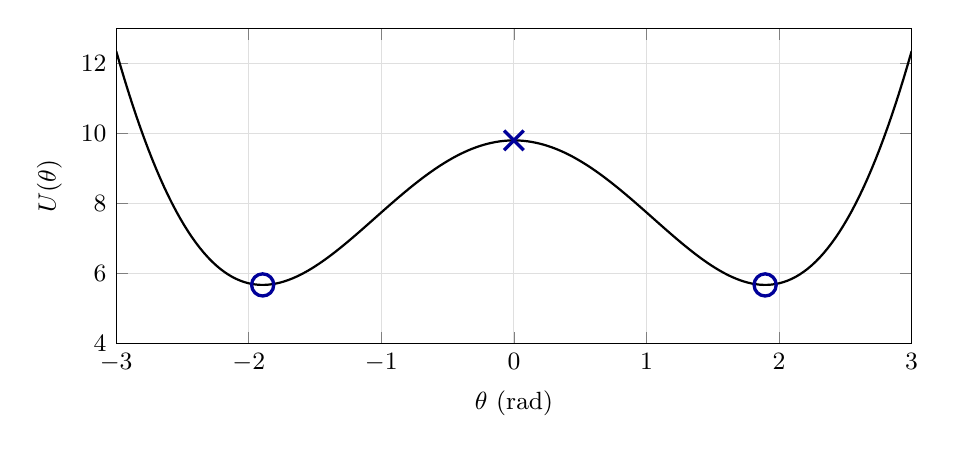
\begin{tikzpicture}
\begin{axis}[
    width=4.6in, height=2.2in,
    xmin=-3, xmax=3, ymin=4, ymax=13,
    xlabel={$\theta$ (rad)}, ylabel={$U(\theta)$},
    xtick={-3,-2,...,3},
    grid=major, grid style={gray!25},
    label style={font=\small}, tick label style={font=\small},
]
\addplot[thick, domain=-3:3, samples=200] {9.8*cos(deg(x)) + 0.5*4.9*x^2};
\addplot[only marks, mark=o, mark size=4pt, very thick, blue!60!black] coordinates {(-1.895,5.676) (1.895,5.676)};
\addplot[only marks, mark=x, mark size=5pt, very thick, blue!60!black] coordinates {(0,9.8)};
\end{axis}
\end{tikzpicture}
\end{center}

\begin{solution}
Equilibria are where $dU/d\theta = 0$, corresponding to flat spots or local minima/maxima on the plot above. Local minima, where U is locally convex, are stable, while local maxima, where U is locally concave, are unstable.

\end{solution}

\item In general, knowing $\vec{r}$ and $\vec{\tau}$, why can't $\vec{\tau} = \vec{r} \times \vec{F}$ be solved uniquely for $\vec{F}$? Why is it possible to find the spring force this way in this problem?

\begin{solution}
The cross product discards any component of $\vec F$ parallel to $\vec r$: for any scalar $\lambda$, $\vec r \times (\vec F + \lambda \vec r) = \vec r \times \vec F$. Knowing $\vec r$ and $\vec\tau$ therefore fixes only the component of $\vec F$ perpendicular to $\vec r$, and there are infinitely many forces that produce the same torque.

In this problem, we know the direction of the equivalent spring force at the mass: a torsion spring acts tangentially, along $\hat e_\theta$, which is perpendicular to $\vec r = \ell\,\hat e_r$. (Any radial force is carried by the rod and does not enter the $\theta$ equation.) With the direction known, only the magnitude remains, and $|\vec\tau| = \ell\,|F|$ gives
\[
\vec F_{\text{spring}} = -\frac{k\theta}{\ell}\,\hat e_\theta .
\]
\end{solution}

\end{enumerate}

\end{document}
